\subsection{Shell Sort}

\subsubsection{Core concepts}
Shell sort is an enhanced version of insertion sort designed to address the problem of elements being far from their correct positions. Shell sort works by initially sorting elements that are far apart from each other, then progressively reducing the gap between elements to be compared. When gap is 1, it is an insertion-sort with nearly sorted array which makes the final pass much faster. This approach efficiently reduces the problem of elements being far from their correct positions, resulting in a quicker sorting process overall.

\vspace{10pt}

\subsubsection{Step-by-step Explanations}
\begin{itemize}[label=-]
    \item Step 1:Find the gap suitable for array, start by gap is equal to 1, gap multiplicate with 3 then plus 1, repeat this step if gap smaller than n. Then divide gap by 3 to find the largest gap that smaller than n.
    \item Step 2: Sort the elements in certain gap, use the idea of insertion-sort to sort the elements in certain gap ( start from i is equal to gap compare a[i] with a[i – gap]).
    \item Step 3: Divide gap by 3 then repeat step 2 until gap is equal to 1, it is an insertion-sort with the array is nearly sorted.
\end{itemize}

\subsubsection{Complexity Analysis}
\textbf{Time complexity analysis:} 
\begin{itemize}
    \item Best Case: $O(n \log n)$
    \item Average Case: Typically around $O(n^{5/4})$ to $O(n^{4/3})$
    \item Worst Case: $O(n^{3/2})$
\end{itemize}

\textbf{Space complexity analysis:} O(1) because it is an inplaced sorting algorithm

\vspace{10pt}

\subsubsection{Variants and Optimizations}
\textbf{Optimizations:} Depend on the data and the number of elements in array, we can choose suitable gap for having better performance. Two common ways to choose: 

\vspace{5pt}

Gap divide by 3: $..., 121, 40, 13, 4, 1$

\vspace{5pt}

Gap divide by 2: $..., 31, 15, 7, 3, 1$

\vspace{5pt}


\textbf{An example of Shell sort} ~\cite{ref1}

\begin{figure}[h]
    \centering
    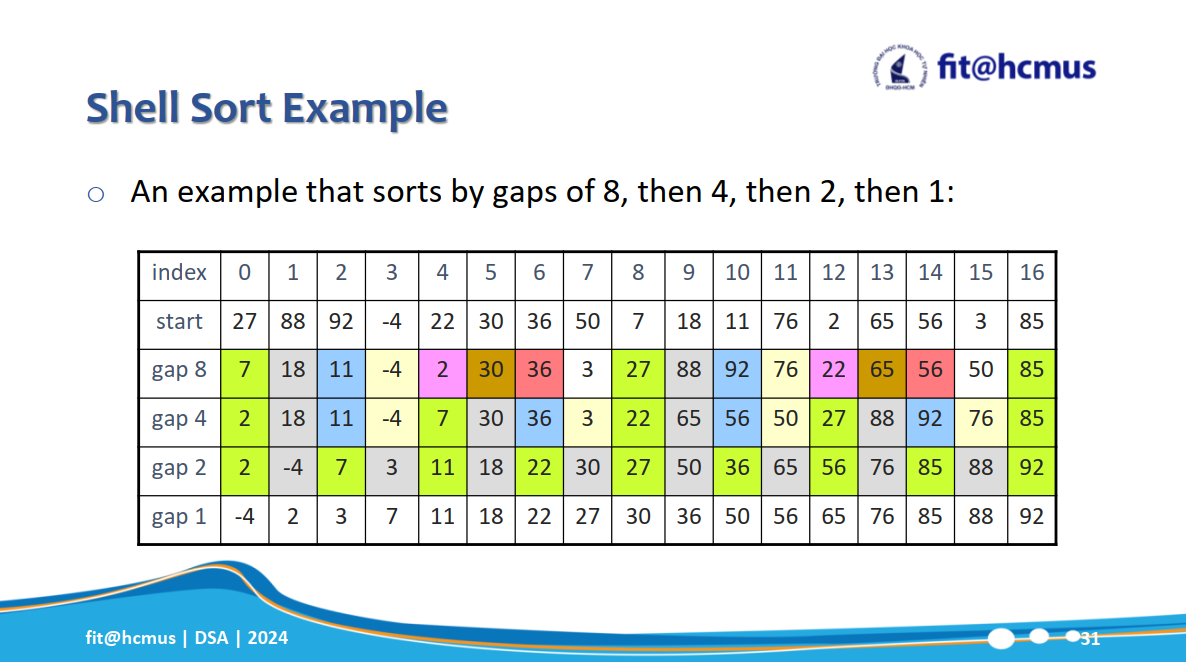
\includegraphics[scale=.23]{Figures/sort_demo/shell.png}
    \caption{Shell Sort Demo}
    \label{fig:enter-label}
\end{figure}